\chapter{Quantum Dots}

\section{One Dimension}

We blast the guy with 
\begin{equation}
    E(t) = E_0\sin^2\left(\frac{t\pi}{T}\right)\cos(\omega t),
\end{equation}
which defines a laser pulse, consisting of several parts. Blah blah blah.

\begin{figure}
    \centering
    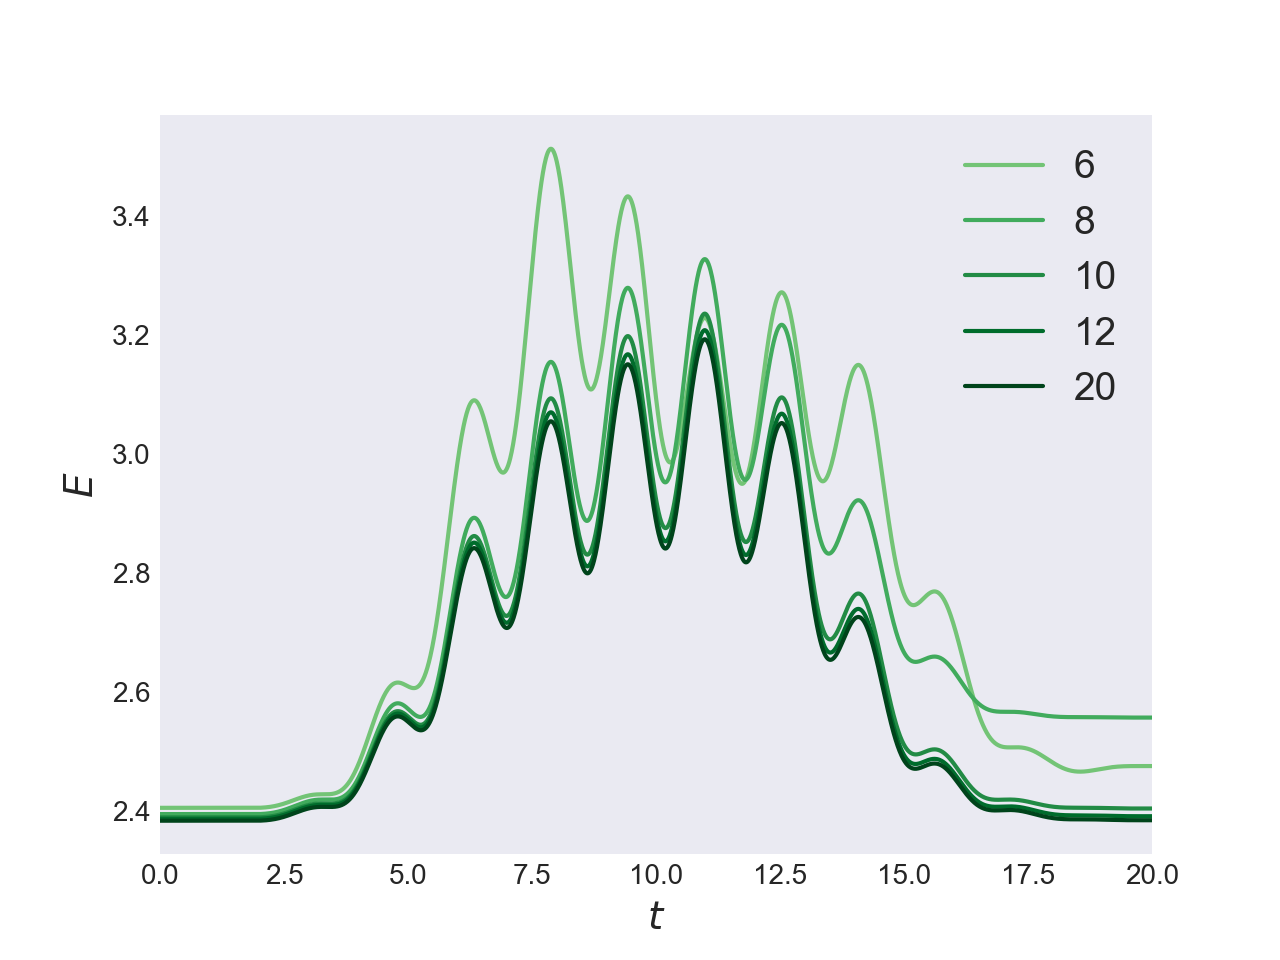
\includegraphics[width=0.8\textwidth]{results/figures/1D/n=2energy.png} 
    \caption{Energy of a one-dimensional quantum dot with $n=2$ electrons
        under the influence of a laser field for different number of spinorbitals
        $l\in\{6,8,10,12,20\}$.
    }
    \label{fig:1d_n2_E}
\end{figure}

\begin{figure}
    \centering
    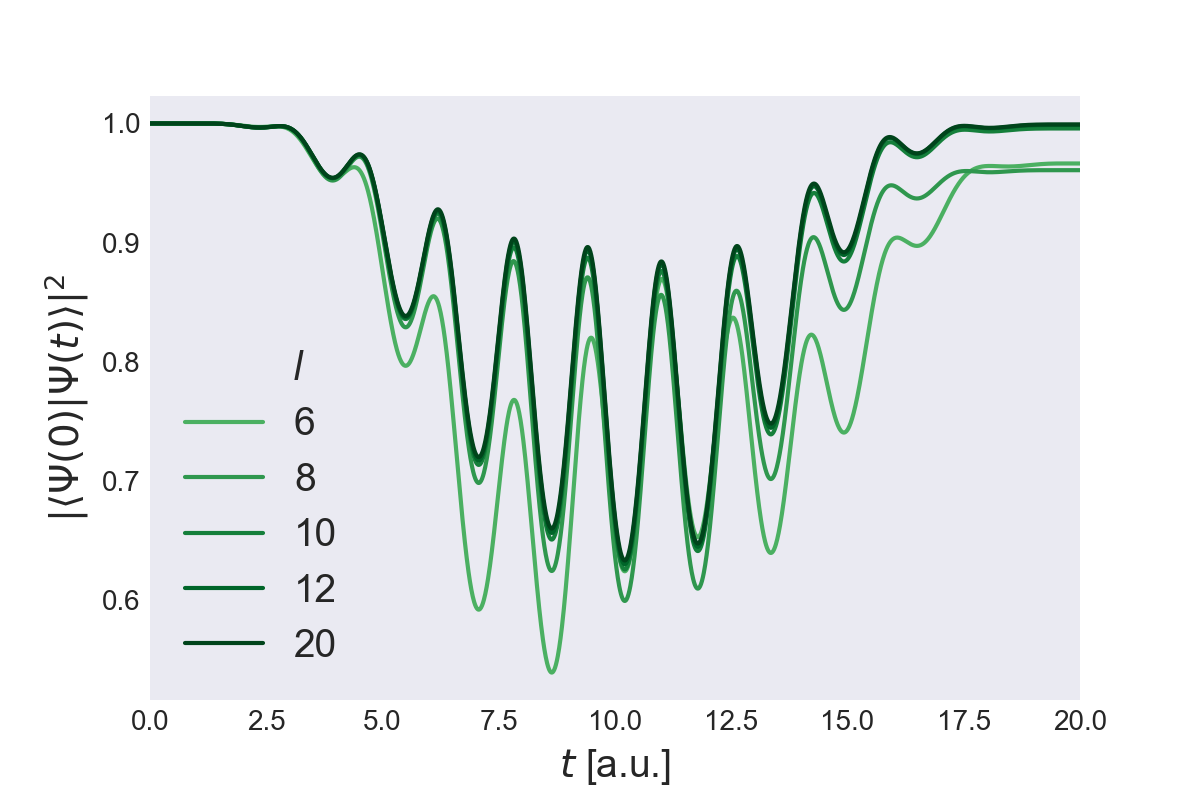
\includegraphics[width=0.8\textwidth]{results/figures/1D/n=2overlap.png} 
    \caption{Probability of being in the ground state $|\braket*{\Psi(0)}{\Psi(t)}|^2$
        for a one-dimensional quantum dot with $n=2$ electrons under 
        the influence of a laser field for different number of spinorbitals 
        $l\in\{6,8,10,12,20\}$.
    }
    \label{fig:1d_n2_overlap}
\end{figure}

\begin{figure}
    \centering
    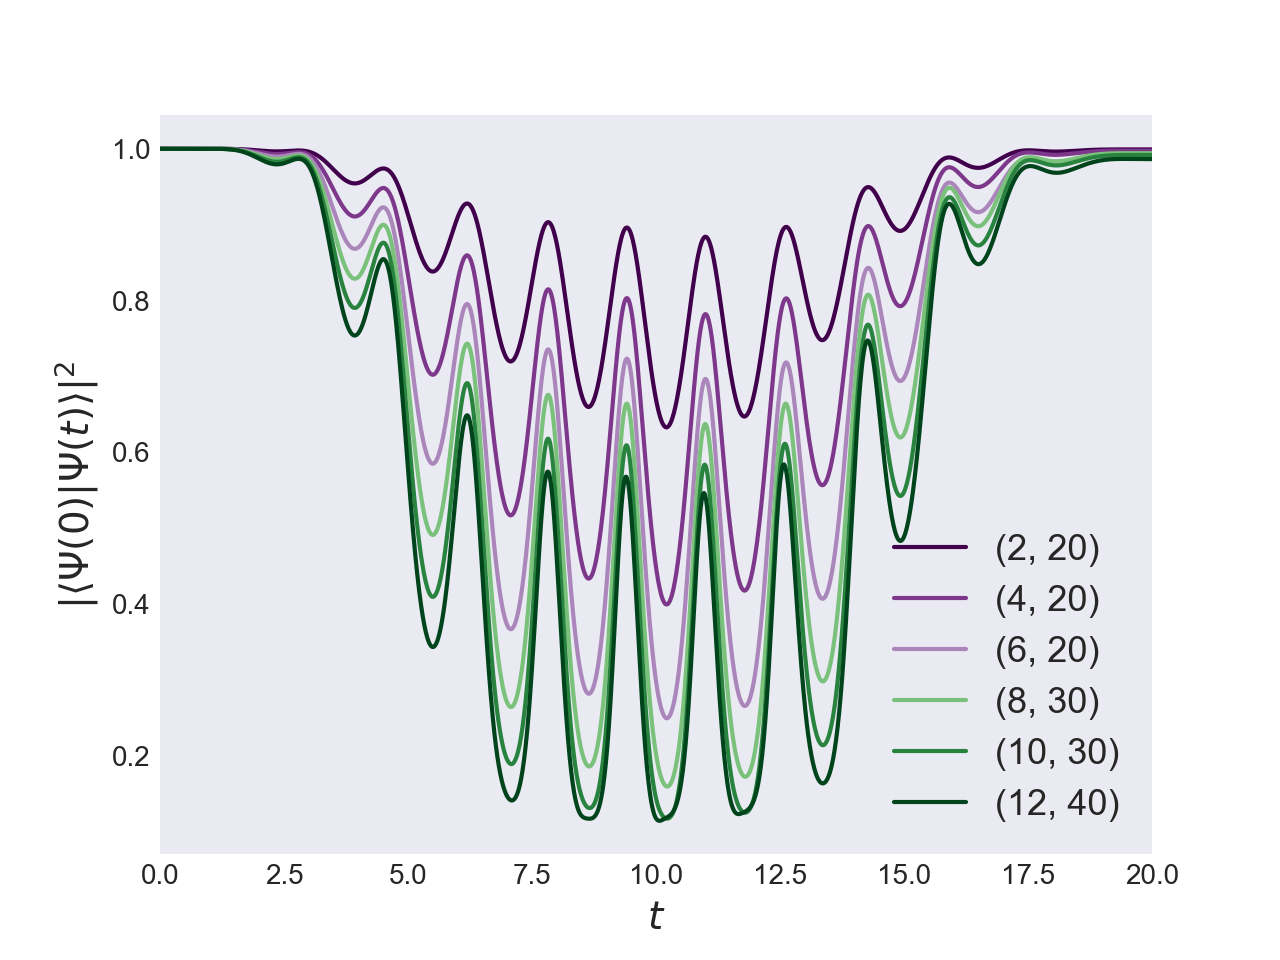
\includegraphics[width=0.8\textwidth]{results/figures/1D/n_compare_overlap.png} 
    \caption{Probability of being in the ground state for $|\braket*{\Psi(0)}{\Psi(t)}|^2$
        for a one-dimensional quantum dot for different number of electrons 
        $n\in\{2,4,6,8,10,12\}$.
    }
    \label{}
\end{figure}

\begin{figure}
    \centering
    \makebox[\textwidth][c]{
    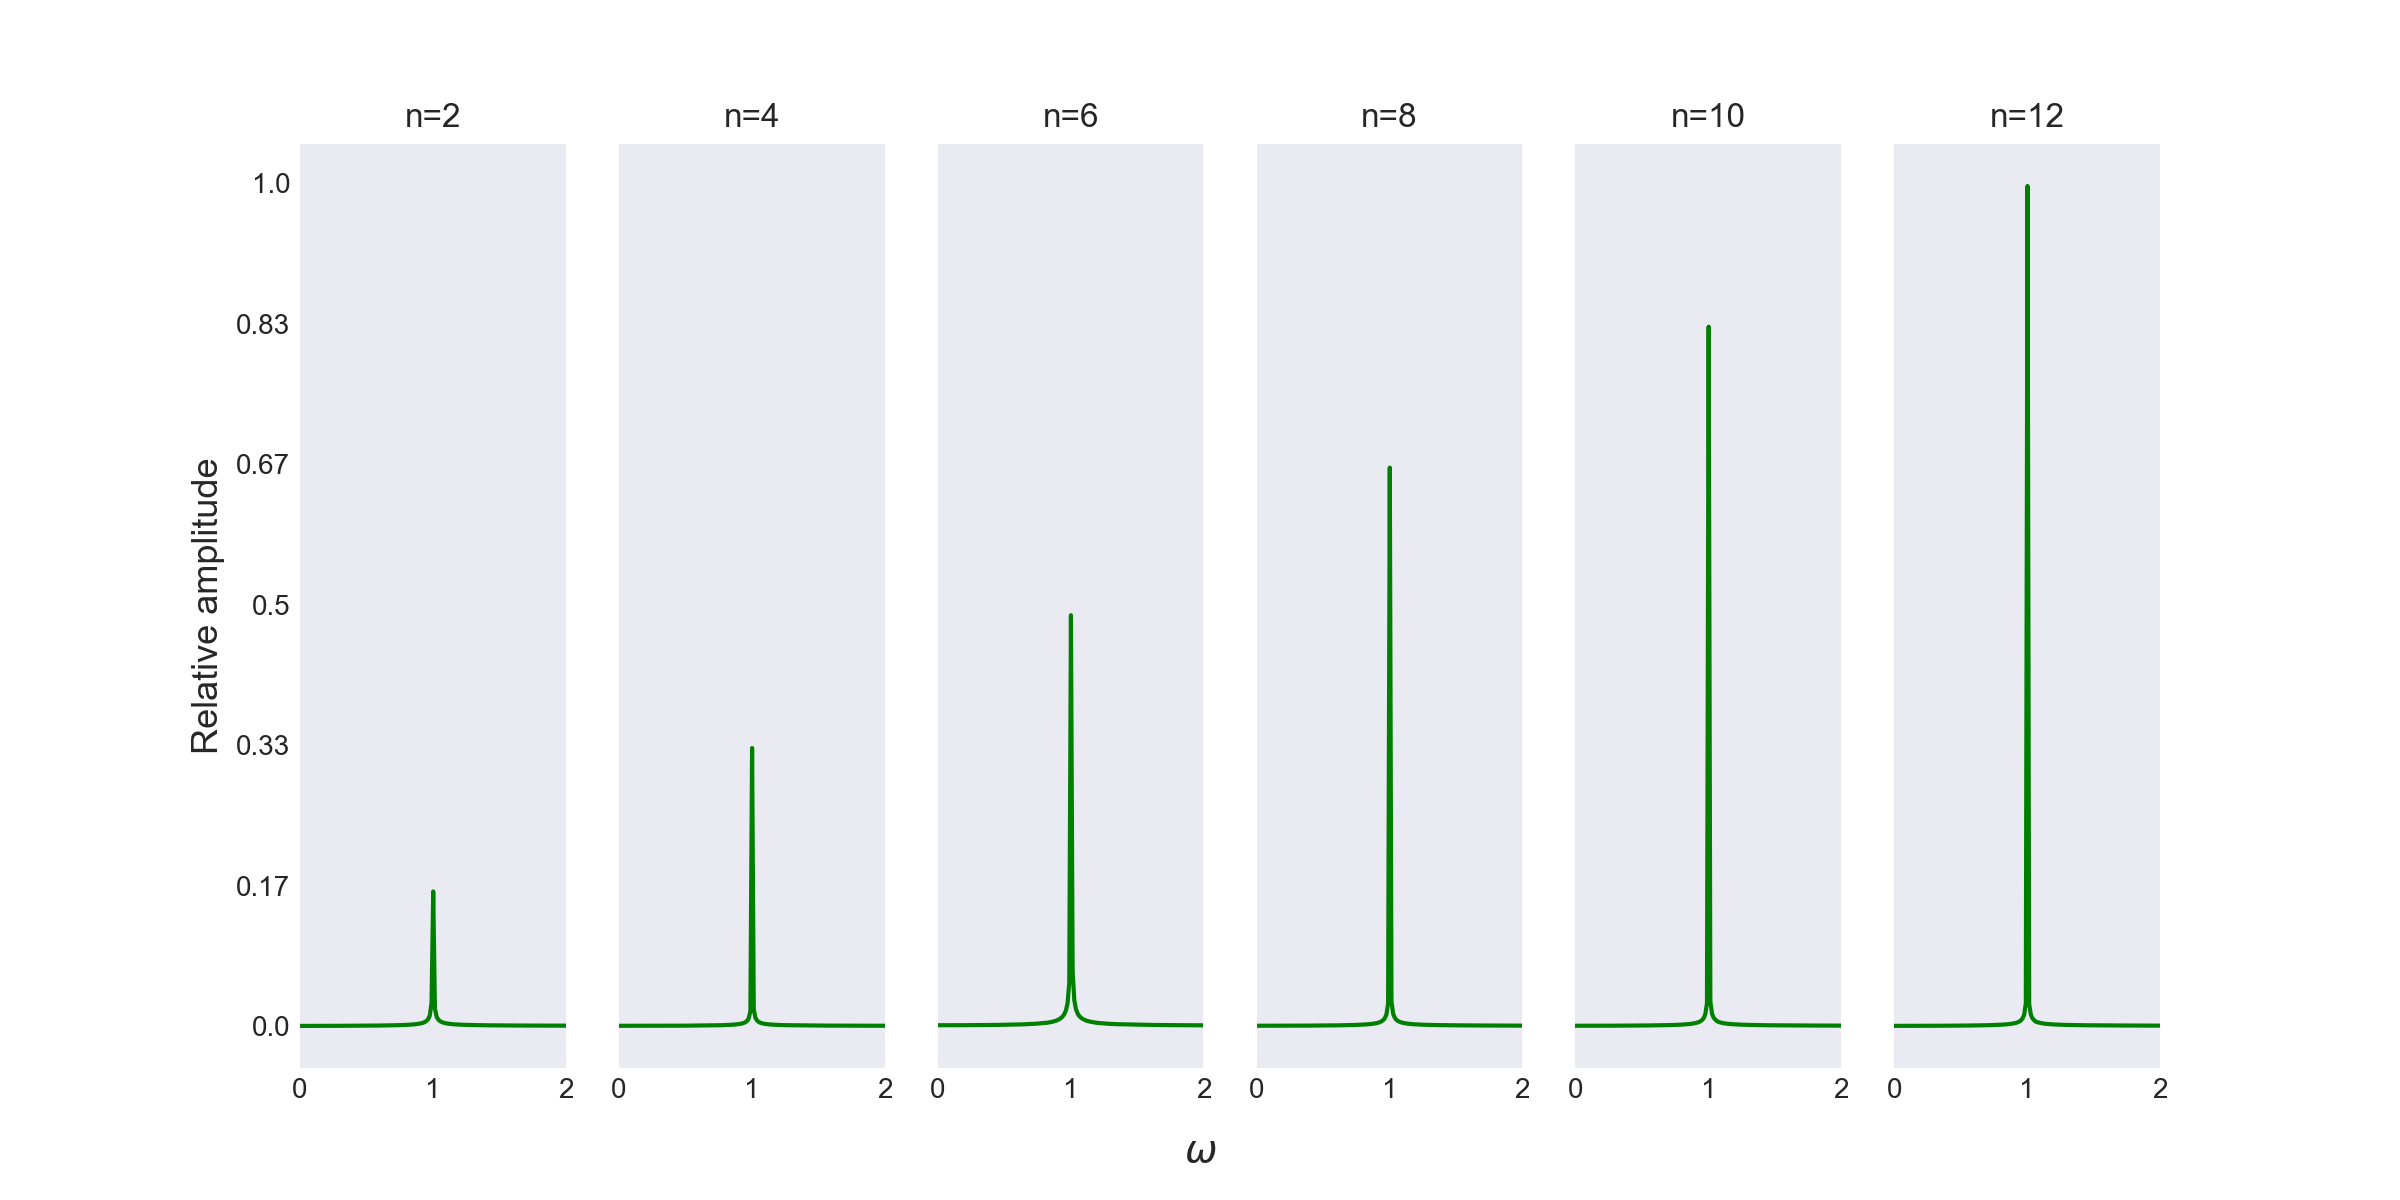
\includegraphics[width=1.4\textwidth]{results/figures/1D/1d_spectrum.png} 
    }
    \caption{Fourier transform of expected value of dipole moment for 
        a one-dimensional quantum dot with different number of electrons
        $n\in\{2,4,6,8,10\}$.
    }
    \label{}
\end{figure}
